\documentclass{beamer}
\usepackage[utf8]{inputenc}
\usetheme{Warsaw}
\title{Biologicky motivované\\výpočtové modely}
\author{Michal Kováč}
\institute{FMFI UK}
\date{24.6.2013}
\begin{document}

\begin{frame}[t]
\titlepage
\end{frame}

\section*{Outline}
\begin{frame}
\tableofcontents
\end{frame}

\section{Biologicky motivované výpočtové modely} % (fold)
\label{sec:biologicky_motivovane_vypoctove_modely}

\begin{frame}[t]\frametitle{Biologicky motivované\\výpočtové modely}
\begin{itemize}
  \item Neurónové siete (od 1943)
  \item Celulárne automaty (od 1948)
  \item Evolučné algoritmy (od 1954)
  \item L systémy (od 1968)
  \item P systémy (od 1998)
  \item \dots

\end{itemize}
\end{frame}

% section biologicky_motivovane_vypoctove_modely (end)

\section{P systém} % (fold)
\label{sec:membranov_systemy}


\begin{frame}[t]\frametitle{Membránová štruktúra}
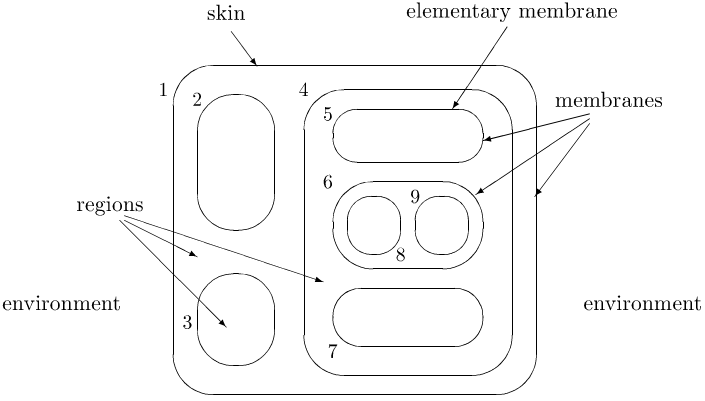
\includegraphics[width=0.7\textwidth]{membrane_structure.png}
\hfill
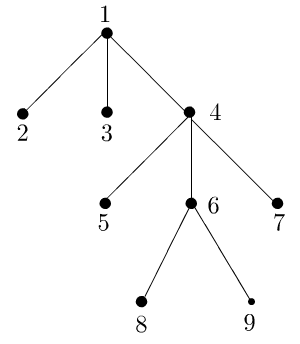
\includegraphics[width=0.3\textwidth]{membrane_tree.png}
\end{frame}

\begin{frame}[t]\frametitle{Obsah membrány}
\begin{itemize}
  \item multimnožina objektov
  \item prepisovacie pravidlá
\end{itemize}
\end{frame}

\begin{frame}[t]\frametitle{Prepisovacie pravidlá}
\begin{itemize}
  \item $a\ |\ b\ |\ b\rightarrow a\ |\ a\downarrow\ |\ a\uparrow\ |\ b\downarrow_6$
  \item $b \rightarrow a\ |\ \delta$
\end{itemize}
\end{frame}

\begin{frame}[t]\frametitle{P systém}

P systém je štvorica $(V, \mu, w_1, w_2,\dots , w_m, R_1, R_2, \dots , R_m)$, kde:
\begin{itemize}
  \item $V$ je abeceda objektov
  \item $\mu$ je membránová štruktúra
  \item $w_1, w_2, \dots w_m$ sú počiatočné multimnožiny v membránach $1\dots m$
  \item $R_1, R_2, \dots , R_m$ sú množiny prepisovacích pravidiel v membránach $1\dots m$.
\end{itemize}

\end{frame}

\begin{frame}[t]\frametitle{Konfigurácia a krok výpočtu}
\begin{itemize}
  \item konfigurácia = membránová štruktúra + obsahy membrán
  \item krok výpočtu: maximálny paralelizmus
\end{itemize}

\begin{itemize}
  \item $a\ |\ b\ |\ b\rightarrow a\ |\ a\downarrow\ |\ a\uparrow\ |\ b\downarrow_6$
  \item $b \rightarrow a\ |\ \delta$
\end{itemize}
\end{frame}


% section membranov_systemy (end)

\section{Varianty} % (fold)
\label{sec:varianty}

\begin{frame}[t]\frametitle{Varianty obsahu membrány}
\begin{itemize}
  \item worm objects
  \begin{itemize}
    \item namiesto multimnožín objektov sú v membránach multimnožiny stringov
    \item inšpirované DNA
  \end{itemize}
\end{itemize}
\end{frame}

\begin{frame}[t]\frametitle{Varianty pravidiel}
\begin{itemize}
  \item kontextové
  \item kooperatívne
  \item katalytické
  \item bezkontextové
  \item s inhibítormi / promótermi
  \item inhibícia pravidiel
  \item bez povolenia rozpúštania membrán
  \item s vytváraním nových membrán
\end{itemize}
\end{frame}

\begin{frame}[t]\frametitle{Varianty kroku výpočtu}
\begin{itemize}
  \item maximálny paralelizmus
  \item sekvenčný
  \item asynchrónny
  \item minimálny paralelizmus
  \item n-paralelizmus
  \item bez priorít
\end{itemize}
\end{frame}

\begin{frame}[t]\frametitle{Iné varianty}
\begin{itemize}
  \item priestorové P systémy
  \item rozpadajúce sa objekty
  \item energie
\end{itemize}
\end{frame}

% section varianty (end)

\section{Plán} % (fold)
\label{sec:plan}

\begin{frame}[t]\frametitle{Plán}
\begin{itemize}
  \item Preskúmať možnosti kombinovania variantov P systémov z hľadiska výpočtovej sily
  \item Porovnať s inými formalizmami, napríklad Petriho siete / reaction systems / CLS / ...
  \item Nájsť nové varianty
\end{itemize}
\end{frame}

\begin{frame}[t]\frametitle{Možnosti kombinovania variantov}
\begin{itemize}
  \item Výpočtová sila
  \item Varianty pravidiel
  \begin{itemize}
    \item kontextové (PsRE)
    \item kooperatívne (PsRE)
    \item katalytické (PsRE)
    \item bezkontextové (PsCF)

    \item bezkontextové s inhibítormi (PsRE)
  \end{itemize}
\end{itemize}
\end{frame}

\begin{frame}[t]\frametitle{Sekvenčné P systémy}
\begin{itemize}
  \item nie sú univerzálne
  \item na univerzalitu treba:
  \begin{itemize}
    \item povoliť neobmedzené vytváranie membrán
    \item inhibítory
    \item iné rozšírenia (vacuum, ...)
    \item inšpirácie z výsledkov iných formalizmov
  \end{itemize}
\end{itemize}
\end{frame}

\begin{frame}[t]\frametitle{Inšpirácie z Petriho sietí}
\begin{itemize}
  \item nie sú univerzálne
  \item s inhibítormi áno
  \item ake ine varianty Petriho sieti este nikto nevyskusal aplikovat v P systemoch?
\end{itemize}
\end{frame}

\begin{frame}[t]\frametitle{Nové varianty}
Dobrý variant by mal byť:
\begin{itemize}
  \item realistický
  \item univerzálny
  \item iredundantný
\end{itemize}
\end{frame}

% section plan (end)

\begin{frame}[plain]
\begin{center}
  Ďakujem za pozornosť
\end{center}
\end{frame}

\end{document}